\documentclass{article}
\usepackage{graphicx}

\title{Project 1 Answers}
\date{2020-06-29}
\author{Edward Wang, Atishay Mitra, Kyle Love}

\begin{document}
\maketitle

\section{Part 1}
a. Since the agent can only observe its 4 adjacent cells, it will choose to move to the east in the first step since the cell to the east is unblocked and is currently the first step on the shortest path to the target state. After the agent would move to position E3, it would observe that the north and east cells are blocked and adjust its path. 

b. In a finite gridworld, there will be a limited number of cells which the agent must check and therefore the time required to find the path or conclude that a path to the target does not exist will be finite. The time it takes to search is linked to the finite number of cells. In contrast, a search algorithm applied on an infinite, constantly expanding gridworld could take an infinite amount of time to conclude whether an agent can reach its target or not.

The number of moves the agent can make is bounded from above by the number of unblocked cells squared because if an adjacent cell is blocked then the agent will backtrack to the same cell at most one time meaning that they will have visited the cell at most two times within the algorithm before either realizing that there is another path or that there is no path at all to the target. 

\section{Part 2}

\section{Part 3}
To test and compare the performance of Repeated Forward A* against Repeated Backward A*, we conducted runs of the algorithms once on each of the fifty grid worlds generated. Firstly, we applied Forward A*, randomly choosing nodes for both the goal and start, then swapped those same nodes and ran it again to simulate Backward A*. We then took the resulting values for the number of expanded nodes and compared them to determine their efficiency. Below are example runs, and the percent difference between the different algorithms in terms of nodes expanded.
\begin{figure}
	\caption{Example Forward A* path: Yellow denotes goal and start}
	\centering
	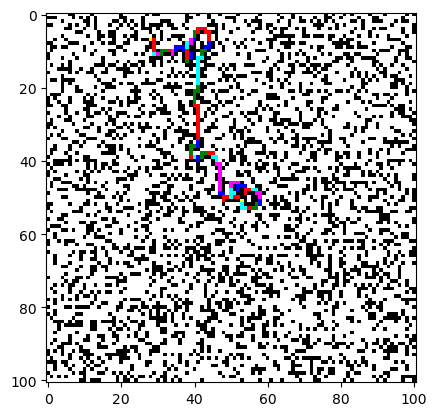
\includegraphics[scale=0.75]{visF}
\end{figure}
\begin{figure}
	\caption{Example Backward A* path}
	\centering
	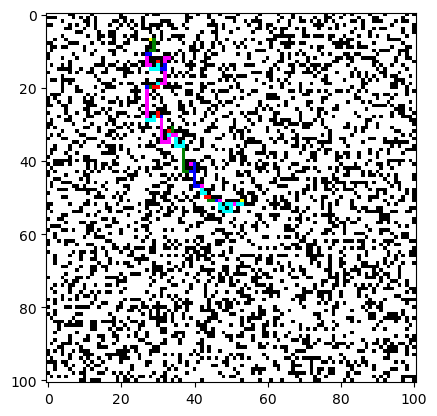
\includegraphics[scale=0.75]{visB}
\end{figure}
\begin{center}
	\begin{tabular}{|c|c|c|}
		\hline
		Percent Difference & Forward A* & Backward A* \\
		\hline
		60.6\% & 816 & 508 \\
		62.8\% & 482 & 296 \\
		-20.8\% & 19 & 24 \\
		-44.2\% & 829 & 1487 \\
		12.8\% & 2024 & 1793 \\
		-36.5\% & 453 & 713 \\
		246\% & 1974 & 517 \\
		56.4\% & 341 & 218 \\
		20.6\% & 262 & 330 \\
		-42.2\% & 1783 & 3086 \\
		\hline
	\end{tabular}
\end{center}

On average, we determined that Forward A* had a runtime 19.66\% lesser that that of Backward A* for the same grids and nodes. Overall, the data seems to suggest that Forward A* is more efficient that Backward A*. However, it is also important to note that, in theory, the two algorithms should have similar performance, given that the obstacles/blocked nodes should hypothetically be spaced randomly. The results we have found are may be largely due to our small sample size. As such, it is hard to conclude off of our data that Forward A* is in fact slower than Backward A*.
\section{Part 4}
\subsection{Manhattan distances}
The manhattan distance is calculated with the following formula
\begin{equation}
	h(s) = |X_s - X_{goal}| + |Y_s - Y_{goal}|
\end{equation}
To be considered a consistent heuristic, it must prove true for the following formula
\begin{equation}
	h(s) <= h(s')+c(s,a,s')
\end{equation}
 We substitute all instances of h(s) and h(s') with the corresponding manhattan distance definition.
\begin{equation}
	|X_s - X_{goal}| + |Y_s - Y_{goal}| <= |X_s' - X_{goal}| + |Y_s' - Y_{goal}| + c(s,a,s')
\end{equation}
Then simplify
\begin{equation}
	|X_s - X_{goal}| + |Y_s - Y_{goal}| - |X_s' - X_{goal}| + |Y_s' - Y_{goal}| <= c(s,a,s')
\end{equation}
Say s and s' are neighboring cells, s' being the immediate successor of the initial state. Furthermore, let us say that s' is vertically adjacent to s. Hence, the following proves true.
\begin{equation}
	|X_s - X_{goal}| - |X_s' - X_{goal}| = 0	
\end{equation}
\begin{equation} 
	|Y_s - Y_{goal}| - |Y_s' - Y_{goal}| = 1
\end{equation}
\begin{equation} 
	|Y_s - Y_s'| = 1
\end{equation}
\begin{equation} 
	|Y_s - Y_{goal}| - |Y_s' - Y_{goal}| = c(s,a,s')
\end{equation}
\begin{equation} 
	h(s) - h(s') = |Y_s - Y_{goal}| - |Y_s' - Y_{goal}|
\end{equation}
Then, given the following inequality
\begin{equation}
	|A| - |B| <= |A-B|
\end{equation}
we say
\begin{equation}
	h(s) - h(s') <= |(Y_s - Y_{goal}) - (Y_s' - Y_{goal})|
		= 1
		= c(s,a,s')
\end{equation}
Therefore, manhattan distances can be said to be consistent heuristics.
\subsection{Adaptive A*}
To prove conclusively that Adaptive A* leaves heuristics consistent over iterations, we must prove it's validity for the following three cases
\subsubsection{In the case both s and s' are expanded}
The new heuristics for both of the nodes are as follows
\begin{equation}
h_{new}(s) = g(s_{goal})-g(s)
\end{equation}
\begin{equation}
h_{new}(s') = g(s_{goal})-g(s')
\end{equation}
We then substitute them into the consistency inequality like so
\begin{equation}
h_{new}(s) <= h_{new}(s')+c(s,a,s')
\end{equation}
\begin{equation}
g(s_{goal}) - g(s) <= g(s_{goal}) - g(s') + c(s,a,s')
\end{equation}
\begin{equation}
g(s') <= g(s) + c(s,a,s')
\end{equation}
Using the above equation, we can conclusively state that the heuristic remains consistent because the algorithm calculates the g value of the successor state based off of the g value of its predecessor with the cost to transition added, so the inequality will never be false.
\subsubsection{In the case s, but not s' is expanded}
The consistency inequality we want to prove in this case is as follows
\begin{equation}
h_{new}(s) <= h(s') + c(s,a,s')
\end{equation}
Firstly, considering that case 1 holds true, we can similarly say that case 2 holds true, because the inequality would still be valid if the node were to be expanded. Nothing changed with regards to the situation, only the amount of information we have has changed. 
Furthermore,
\begin{equation}
f(s) <= f(s')
\end{equation}
because the algorithm prioritizes the smallest f-value to expand nodes. Therefore, if we substitute into the equation above as follows, splitting the f-value into h+g values,
\begin{equation}
	h_{new}(s) + g(s) <= h(s') + c(s,a,s') + g(s)
\end{equation}
we find that 
\begin{equation}
h_{new}(s) <= h(s') + c(s,a,s')
\end{equation}
proving the inequality true
\subsubsection{In the case neither are expanded}
Unlike the other cases, the adaptive A* algorithm modifies neither s or s', so considering the fact that the consistency inequality should hold true in normal A*, we can conclude that this case holds true as well.
\section{Part 5}
To test Adaptive A* against Forward A*, we underwent a similar process to the Backward A* vs Forward A* trials, comparing the Adaptive A* algorithm for the same nodes as the initial Forward A* trials to determine which of them was the more efficient. A sample of ten of the trials and an example comparison between paths is shown below.
\begin{figure}
	\caption{Example Forward A* path: Yellow denotes goal and start}
	\centering
	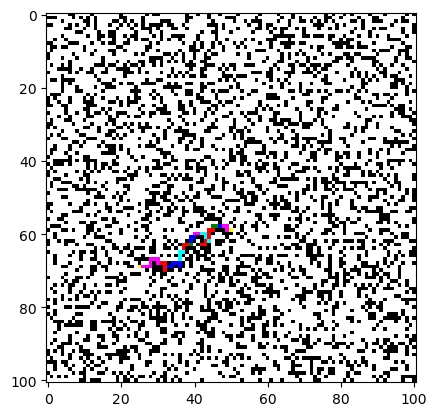
\includegraphics[scale=0.75]{visF2}
\end{figure}
\begin{figure}
	\caption{Example Adaptive A* path}
	\centering
	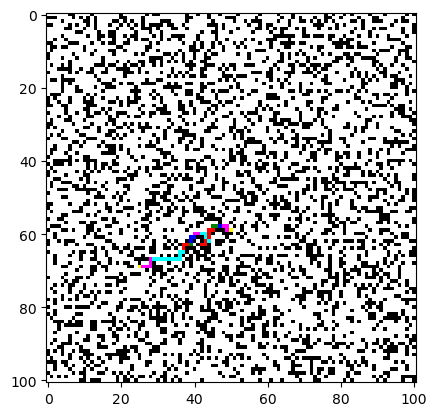
\includegraphics[scale=0.75]{visA}
\end{figure}
\begin{center}
	\begin{tabular}{|c|c|c|}
		\hline
		Percent Difference & Forward A* & Adaptive A* \\
		\hline
		6.1\% & 2690 & 2527 \\
		-463.5\% & 2318 & 13062 \\
		0.8\% & 2277 & 2258 \\
		-131.4\% & 1349 & 3122 \\
		-395.3\% & 495 & 2452 \\
		-49.6\% & 679 & 1016 \\
		-13.2\% & 930 & 1053 \\
		2.8\% & 528 & 513 \\
		-17.9\% & 756 & 891 \\
		-51.6\% & 1719 & 2606 \\
		\hline
	\end{tabular}
\end{center}
As can be seen, our implementation of Adaptive A* is somewhat inconsistent in runtime. In some of the cases, it makes improvements on the original, but in most others, the runtime far exceeds a typical Forward A* implementation. There are a number of possible reasons for this. The most likely would be that the implementation itself was incorrect and possessed some small errors that led to inconsistencies in performance. In coding, the algorithm was difficult to debug, and after a certain point, it felt as if there was no proper way to optimize further. However, there is also the possibility that this is simply not it's usage case, considering that Adaptive A* is said to handle moving goals best. Either way, this section of the project can only be inconclusive on whether or not Adaptive A* is truly superior to Forward A*.

\section{Part 6}
Each node in our implementation has the following members: x, y, costToGo, costToCome, parent, blocked, search, and action\_cost. X and Y may each take 7 bits (int up to 127) to implement considering the size of the gridworld (101), while costToGo and costToCome should each require 8 bits(int up to 255), taking into account the longest path with a manhattan heuristic should be around 200 nodes in length. Tree pointers should take 2 bits(int up to 3) to account for surrounding nodes. Blocked is a one bit boolean, and considering action\_cost is based off of it, we can do away with that all together. The search member is somewhat difficult to estimate for, but for leeway, we grant it 8 bits(int up to 255) Overall, each node should take 41 bits.

Secondly, the open list is a heap, implemented with the following members: size, maxsize, and array. Size and maxsize should both be around 14 bits(int up to 18384), accounting for the size of the gridworld (10000). The array is a pointer reference(32 bits) pointing to a block of memory of length maxsize. References in the array to access each node can use the x,y coordinates, so each reference can be 14 bits in size. Therefore, the size of the array is 32+maxsize*14 bits. In this case, we doubled the maxsize every time size equaled it, but memory usage can be decreased if the program properly anticipates and adjusts max size in advance of entries entering the heap. Overall an optimal heap should just be 32+maxsize*14(max 10201) bits, considering we don't need size to keep track of anything.

The closed list was implemented as a simple array. 32 bits for the initial reference to the block of memory, 14 bits for each reference to a node. Each entry is appended to the end, so it is essentially 32+14*expanded(max 10201) bits

In addition, we also stored the path nodes in an array, resulting in 32 bits for the initial reference and 14*len(path) (max 200) bits, 32+14*len(path)
Finally, we populated a 2 dimensional array at the beginning of the program for the sake of easy referencing. 32 bits for the initial reference, another 32*101 bits for each of the arrays, then we initialize 101 cells with their own nodes. Because the other data structures reference this grid for node information, each cell must also have a 32 bit reference. Hence, the overall memory usage is 32+32*101+10201*(32+41), resulting in a figure of 747937 bits. Optimally, we should've read directly from the file at each point and built nodes as we discovered them.

Assuming the worst case scenario, for a grid world of 1001*1001 bits, we would first initialize a 2 dimensional array of 1001*1001, resulting in 32 bits for the initial reference, 32*1001 for each of the arrays, 32+41 for each of the 1001*1001 cells, resulting in a memory usage of 73178137. Given that the open and closed list are mutually exclusive for nodes, we store a memory reference for each of them (32*2), the size variable (14) and maxsize variable (14), and assume that all nodes are in one of the lists, resulting in 1001*1001*14. Hence, a memory usage of about 14092. The path list should be 32+14*(2000) assuming longest path. Overall, we should have a memory usage of about 87234275 bits.

To calculate the largest gridworld usable within 4 MB, we must first simplify the equation. Let the length of the grid world be represented by x. Memory usage is then
\begin{equation}
32+32x+73x^2+32*2+14*2+14x^2+32+14*2(x-1) = M
\end{equation}
Simplified
\begin{equation}
	128+60x+87x^2 = M
\end{equation}
The subsequent equation is quadratic. We substitute 32000000 in for M, considering an MB has 8000000 bits, and solve for x using the quadratic formula. The maximum size of a grid world usable within 4 MB, assuming an optimal memory allocation, is about 606*606.
\end{document}
